\chapter{Coordination and Formation}

\paragraph*{}
This chapter presents the implementation of a swarm path planning system designed to form a coordinated structure around a target object. The formation algorithm computes collision-free trajectories based on the positional data received from each robot, assigning optimized paths, typically the shortest feasible route, to individual swarm members. These paths are then converted into discrete waypoints, a format well-suited for execution by the swarm’s motion controllers, ensuring accurate and efficient formation around the object. The flow for formation planning is illustrated in Figure \ref{fig:path-planning-flow}.

\begin{figure} [H]
    \centering
    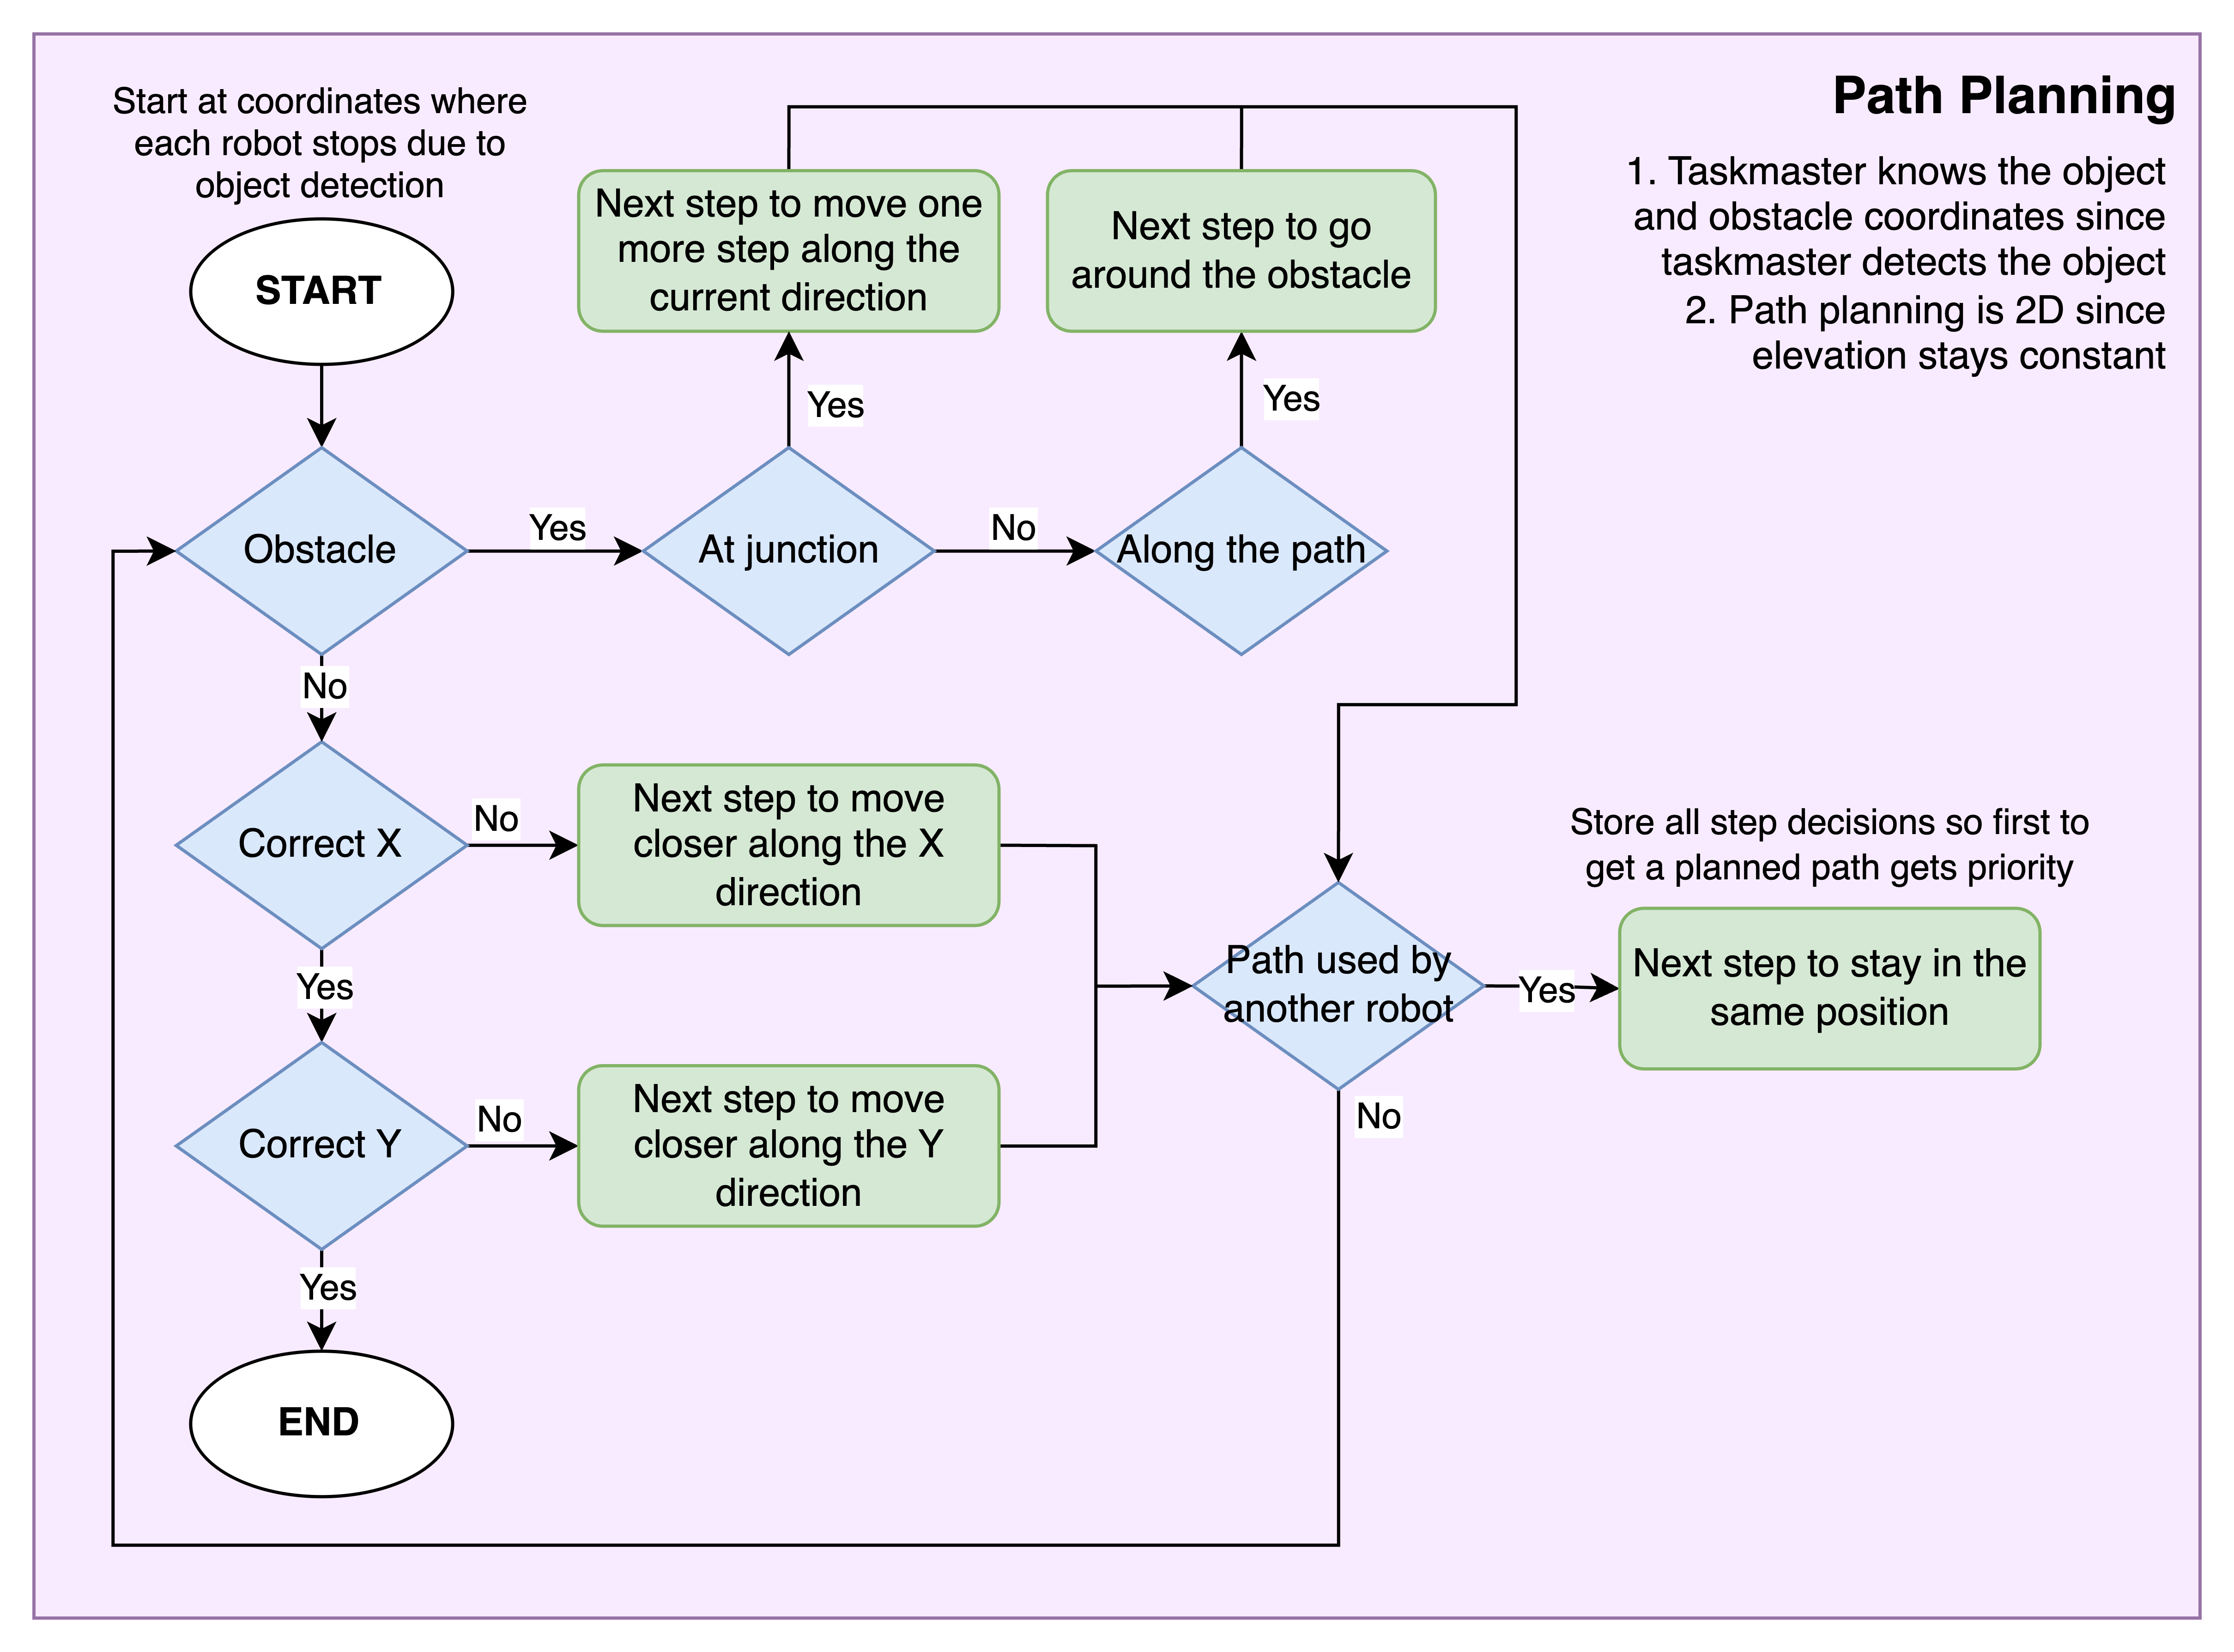
\includegraphics[width=1\linewidth]{assets/images/formation/path-planning-flow.png}
    \caption{Path Planning Flow}
    \label{fig:path-planning-flow}
\end{figure}

\paragraph*{}
In the process of building a swarm formation, computations for the desired coordinates where the swarm units should be moving to (later referenced as \textbf{"target coordinates"}), and the desired path the members can take in order to move towards the goal are essential. The key parameters for this calculation include: the \textbf{radius} where the swarm should place itself around the object, swarm fleet \textbf{member count}, \textbf{current coordinates} for the swarm, and target \textbf{object coordinates}.

\paragraph*{}
The member count is a vital initial point since it will be used to compute the angle \(\theta\) between each set of target coordinates using the following formula:

\[\theta = (2\pi / n) * i\]

\begin{description}
    \item[where:]
    \item \(\theta\) = angle between each set of target coordinates (in radians)
    \item \(n\) = swarm system member count
    \item \(i\) = member identifier (e.g. 0 to 4 for a swarm fleet of 5 members)
\end{description}

\paragraph*{}
Currently, the formation is determined by utilizing a given radius for the swarm robotic members to attempt to surround. In accordance with the member count providing the angle, the individual target coordinates for each robot can be calculated using an adaptation from the Pythagorean Theorem. 

\[x' = x + rcos\theta\]
\[y' = y + rsin\theta\]

\begin{description}
    \item 
    \item[where:]
    \item \((x, y)\) = robot's present coordinates
    \item \((x', y')\) = target \((x, y)\) coordinates
    \item \(r\) = radius
\end{description}

\paragraph*{}
The target coordinates at this stage would often result in floats; therefore, it is necessary to round the numbers and record the margins of error to snap the coordinates to a grid system. With the resulting calculation of the target coordinates, it is sufficient to proceed to the next stage, which is \textbf{path planning}. The path planning algorithm follows a simple \textbf{"Avoid paths that cause conflicts, but if all paths cause conflicts, pause before continuing"} rule. Hence, recording the paths and the timestep the movement will happen is crucial.

\paragraph*{}
For instance, when the intended movement for robot2 and robot3, there is a conflicting movement in \textit{timestep 2} at the \textit{coordinates (3, 3)}. Therefore, robot3 halts for a single timestep before continuing. This is designed so that robots will not take unnecessary detours and create environmental variabilities.

\paragraph*{}
Moreover, The current implementation of the path planning algorithm also takes into account the presence of obstacles presented by the localization and object detection modules as input. The cases for obstacle appearance and avoidance can be divided into two main categories: obstacles appearing at the \textbf{turning} location while heading to the destination, and obstacles appearing while heading \textbf{straight} towards a destination.

\paragraph*{}
Obstacles appearance during turning can also be considered as the them appearing on a different axis compared to the ongoing movement (robot moving along the x axis, obstacles appear while turning onto the y axis, vice versa). Obstacles encountered this way can be tackled by continuing movement by a single step in the same direction as its ongoing movement, then computing the path as per the usual method. For visualization purposes, this case has been portrayed in Figure \ref{fig:obstacle-avoidance-case-1}.

\begin{figure} [H]
    \centering
    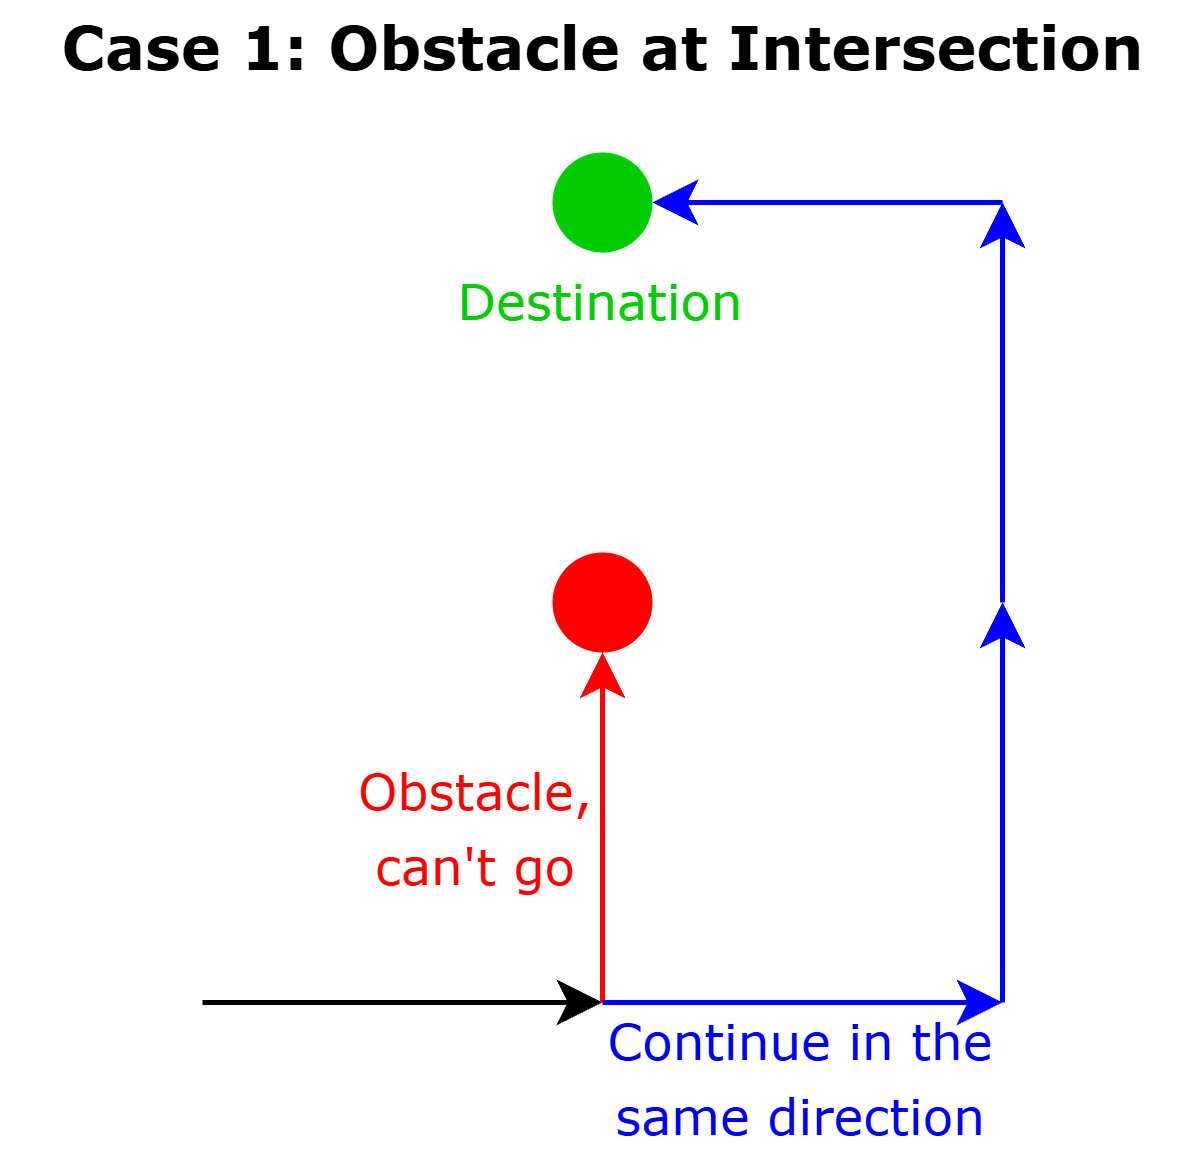
\includegraphics[width=0.55\linewidth]{assets/images/formation/obstacle-avoidance-case1.png}
    \caption{Obstacle Avoidance Case 1: Obstacle during Turning}
    \label{fig:obstacle-avoidance-case-1}
\end{figure}

\paragraph*{}
The other case for obstacle appearance can be considered as one where it coincides with the line of movement the robot is currently ongoing (robot moving along the x axis, obstacles appear along that x path). This case can be handled by "going around" the obstacles, appending movements that go around the obstacles both in the positive and negative directions, and continuing the existing path planning algorithm. Figure \ref{fig:obstacle-avoidance-case-2} illustrates the case and the proposed solution.

\begin{figure} [H]
    \centering
    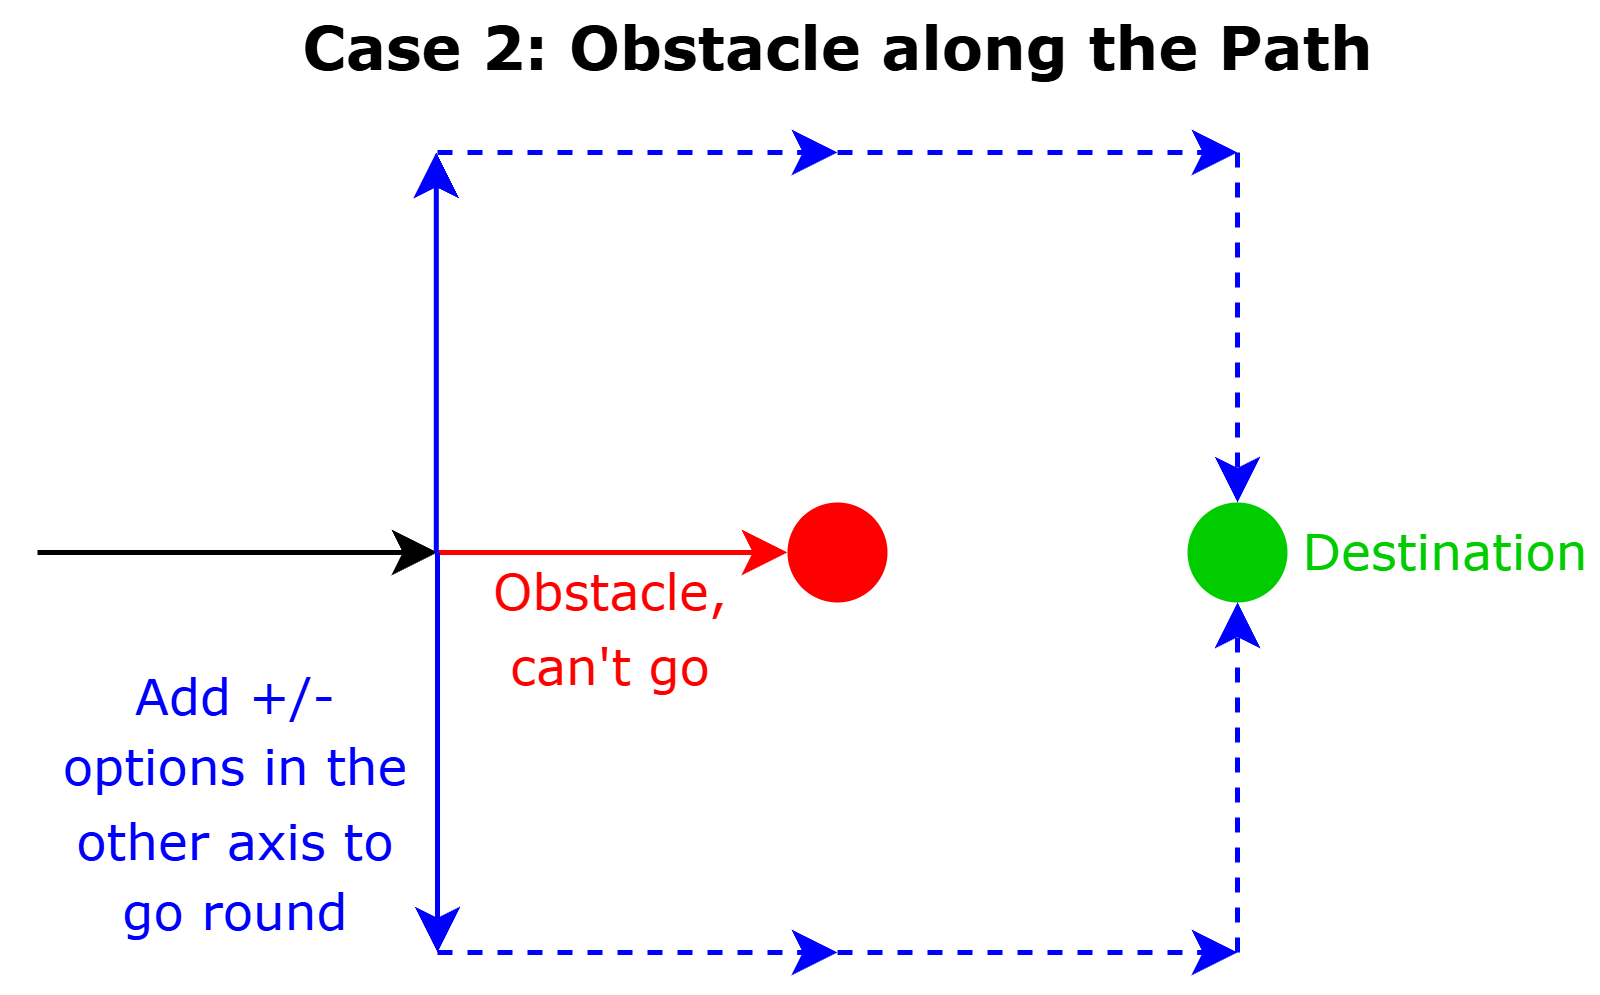
\includegraphics[width=0.75\linewidth]{assets/images/formation/obstacle-avoidance-case2.png}
    \caption{Obstacle Avoidance Case 2: Obstacle along the Current Path}
    \label{fig:obstacle-avoidance-case-2}
\end{figure}

\paragraph*{}
Once the appropriate paths have been computed, there are two essential considerations remaining, namely, formatting them to be compatible with communication and motion controller, and covering actions after arriving at the destinations such as orientations of the robots to grip the objects. An illustration of how these two considerations are tackled is displayed in Figure \ref{fig:path-waypoint}.

\begin{figure} [H]
    \centering
    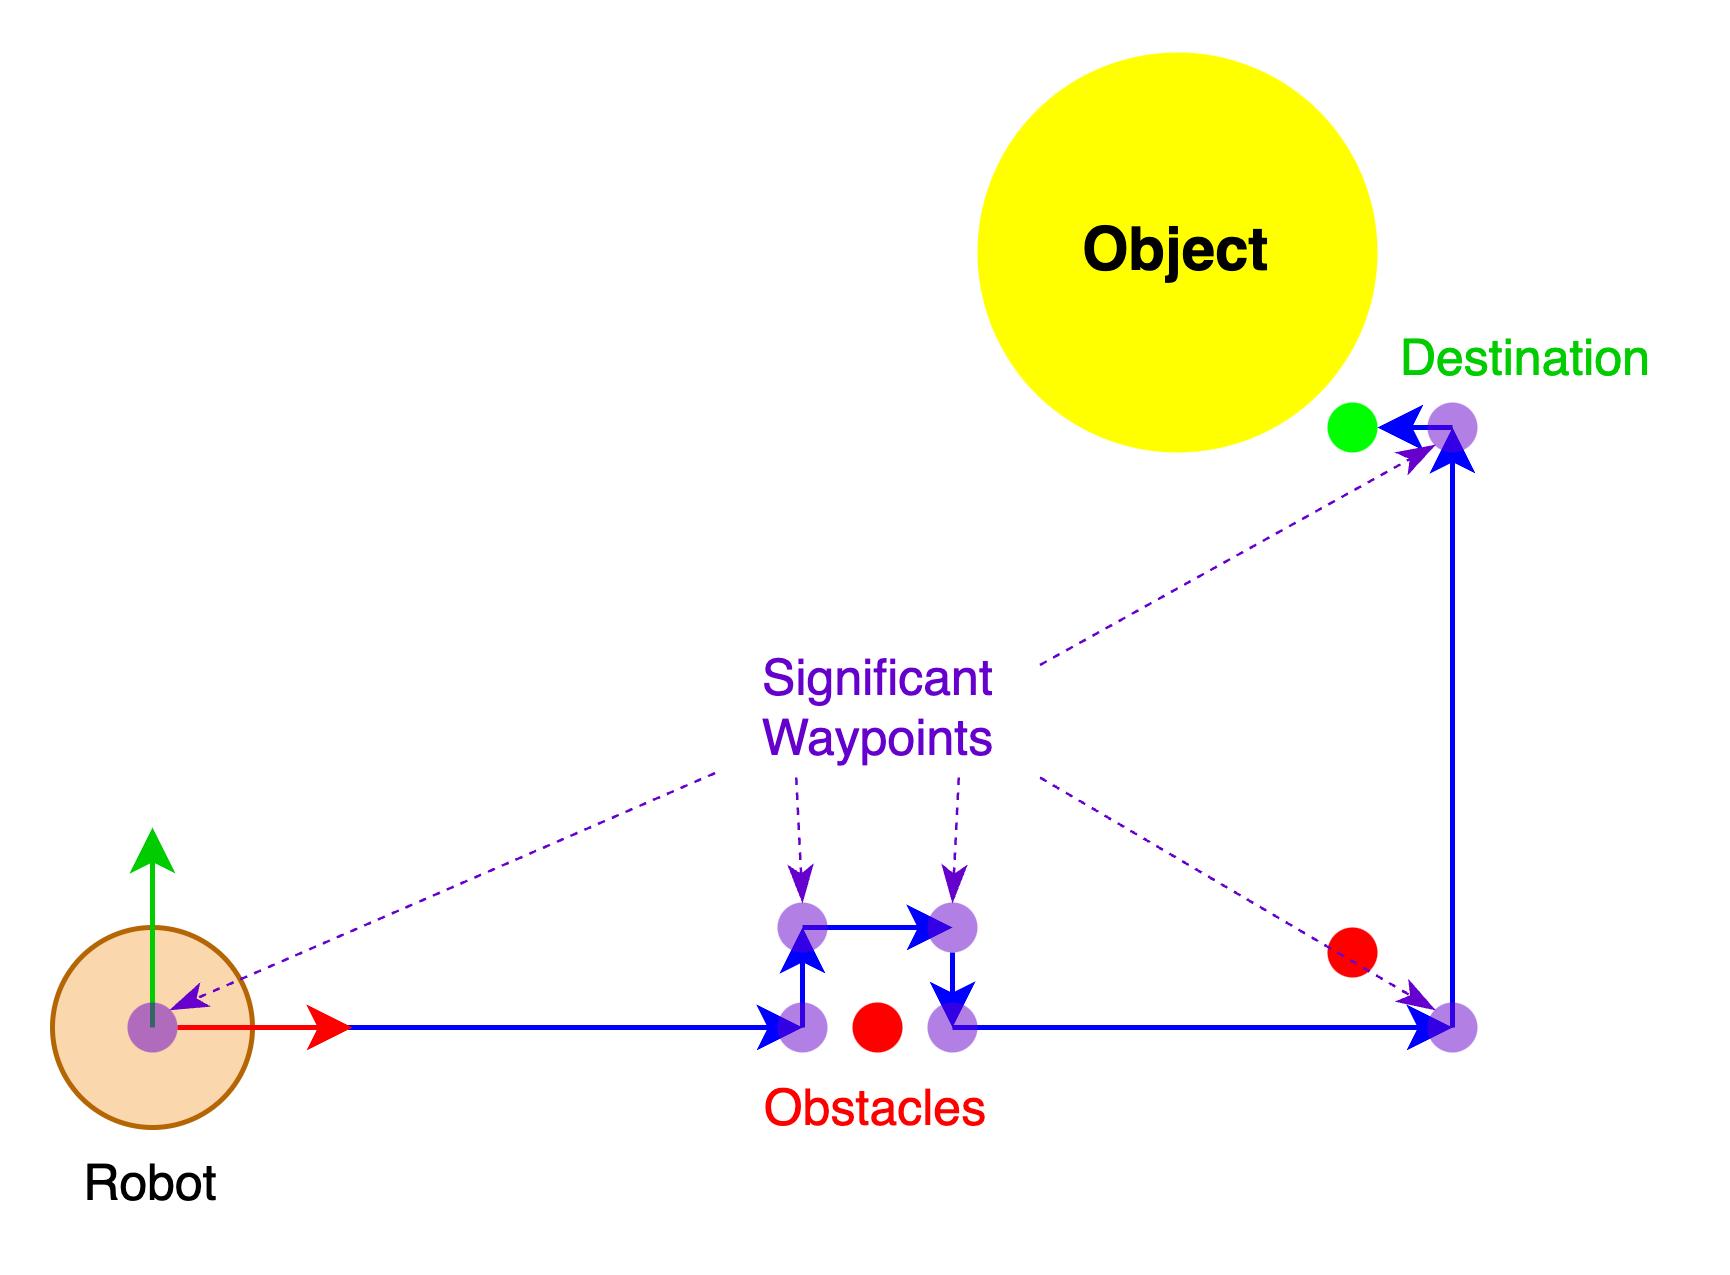
\includegraphics[width=0.7\linewidth]{assets/images/formation/path-waypoint.png}
    \caption{Path Waypoint}
    \label{fig:path-waypoint}
\end{figure}

\paragraph*{}
The computed paths originally lists all coordinates along the paths with a miniscule interval; for long paths, these coordinates can easily reach over a thousand. Considering this with the potential of scalability of swarm systems of numerous robots, this is a glaring weakness. Thus, the paths are translated to discrete waypoints, only recording significant coordinates such as corners for turning, and a repeat of coordinates for momentarily stopping, in case the robot has to wait for another to move past to avoid colliding. This can translate a thousand-long list of coordinates into potentially several tens of them, dependent on the number of corners the robots have to take, making the structure more efficient.

\paragraph*{}
For appropriate path planning, it is also essential to consider the subsequent actions after robots arrive at their destinations in the equilateral formation around the object. In this case, the orientation of the robots have to be considered. Transmitting the final orientations of the robots will allow them to position themselves with the gripper facing toward the detected object, completing the formation and allowing them to move the object. The swarm can also surround the object in a higher actual radius than the object's, position themselves according to the final orientation, and move in to form a sufficient hold. 
